% ============================================================
%  Energy AI Hackathon 2026 — 3-Minute Beamer Presentation
%  Compile with:  pdflatex presentation.tex  (run twice)
%  Theme requires: beamer (standard), pgfplots, booktabs
% ============================================================
\documentclass[aspectratio=169, 10pt]{beamer}

% ── Theme & colours ──────────────────────────────────────────
\usetheme{Madrid}
\usecolortheme{whale}

\definecolor{energyblue}{RGB}{0, 82, 136}
\definecolor{solaryellow}{RGB}{255, 180, 0}
\definecolor{greenok}{RGB}{30, 140, 60}
\definecolor{reddanger}{RGB}{190, 30, 30}
\definecolor{lightgray}{RGB}{245, 245, 245}

\setbeamercolor{palette primary}  {bg=energyblue,  fg=white}
\setbeamercolor{palette secondary}{bg=energyblue!80, fg=white}
\setbeamercolor{palette tertiary} {bg=energyblue!60, fg=white}
\setbeamercolor{palette quaternary}{bg=energyblue,  fg=white}
\setbeamercolor{structure}{fg=energyblue}
\setbeamercolor{block title}{bg=energyblue, fg=white}
\setbeamercolor{block body} {bg=lightgray}
\setbeamercolor{alerted text}{fg=reddanger}

\setbeamertemplate{navigation symbols}{}
\setbeamertemplate{footline}[frame number]

% ── Packages ─────────────────────────────────────────────────
\usepackage{booktabs}
\usepackage{colortbl}
\usepackage{graphicx}
\usepackage{amsmath}
\usepackage{amssymb}
\usepackage{xcolor}
\usepackage{tikz}
\usepackage{pgfplots}
\pgfplotsset{compat=1.18}
\usepackage{eurosym}        % \euro symbol
\usepackage{microtype}
\usepackage{array}
\usepackage{multirow}

% Helper macros
\newcommand{\good}[1]{\textcolor{greenok}{\textbf{#1}}}
\newcommand{\bad}[1]{\textcolor{reddanger}{\textbf{#1}}}
\newcommand{\hl}[1]{\colorbox{solaryellow!40}{#1}}
\newcommand{\Dt}{\Delta t}

% ─────────────────────────────────────────────────────────────
%  TITLE
% ─────────────────────────────────────────────────────────────
\title[Energy AI Hackathon 2026]%
      {\textbf{Smart Battery Dispatch}\\[2pt]
       \large Load Forecasting + LP-MPC Controller}
\subtitle{Energy AI Hackathon 2026}
\author{Team: AI Energy Optimization}
\institute{Sondrio Residential Prosumer --- Italy}
\date{May 2026}

% ─────────────────────────────────────────────────────────────
\begin{document}
% ─────────────────────────────────────────────────────────────

\begin{frame}[plain]
  \titlepage
\end{frame}

% ============================================================
%  SLIDE 1 — FORECASTING MODEL
% ============================================================
\begin{frame}{Slide 1 \hfill \textcolor{gray}{\small$\approx$30 s}}
  \frametitle{Load Forecasting Model}

  \begin{columns}[T]
    % Left column
    \begin{column}{0.52\textwidth}
      \begin{block}{Algorithm: LightGBM Regressor}
        \begin{itemize}
          \item Tree-based model; lag features \textit{are} the time series
          \item Won M5 Competition (42\,000 series) \& GEFCom2014
          \item Trains in $<$5\,s; no vanishing gradients
        \end{itemize}
      \end{block}

      \vspace{4pt}
      \begin{block}{43 Features — Key Groups}
        \renewcommand{\arraystretch}{1.1}
        \small
        \begin{tabular}{ll}
          \textbf{Short lags}   & \texttt{lag\_1} -- \texttt{lag\_16}
                                  (15\,min -- 4\,h) \\
          \textbf{Long lags}    & \texttt{lag\_96, lag\_672, lag\_1344} \\
          \textbf{Momentum}     & \texttt{delta\_1} = $\ell_{t-1}-\ell_{t-2}$
                                  \textit{(top feature)} \\
          \textbf{Rolling}      & mean/std/max over 1\,h -- 1\,week \\
          \textbf{Weather}      & temp, HDD, CDD, cloud cover \\
          \textbf{Calendar}     & sin/cos time, holiday flags \\
        \end{tabular}
      \end{block}

      \vspace{4pt}
      \begin{alertblock}{Two-Phase Training}
        Early-stop on Oct--Dec val
        $\Rightarrow$ retrain on \textit{all} 2024 at fixed depth
        $\Rightarrow$ best\_iter = \textbf{487 trees}
      \end{alertblock}
    \end{column}

    % Right column
    \begin{column}{0.44\textwidth}
      \begin{block}{2025 Test Results}
        \centering
        \renewcommand{\arraystretch}{1.4}
        \begin{tabular}{lc}
          \toprule
          \textbf{Metric} & \textbf{Value} \\
          \midrule
          RMSE  & 0.6811\,kW \\
          MAE   & 0.4537\,kW \\
          \rowcolor{solaryellow!30}
          \textbf{NRMSE} & \textbf{46.14\,\%} \\
          \bottomrule
        \end{tabular}
      \end{block}

      \vspace{6pt}
      \begin{exampleblock}{Why 46\,\% is Expected}
        \small
        Single-household 15-min load:\\
        mean $\approx$1.48\,kW, std $\approx$1.25\,kW\\
        CV $\approx$85\,\% --- stochastic appliances\\
        \textbf{Published range: 35--60\,\% NRMSE}
      \end{exampleblock}

      \vspace{4pt}
      \begin{exampleblock}{Key Insight}
        \small Adding \texttt{lag\_1} (15-min memory):\\
        NRMSE: \bad{67.6\%} $\rightarrow$ \good{46.1\%}\\
        \textit{$-$21\,pp from one feature group}
      \end{exampleblock}
    \end{column}
  \end{columns}
\end{frame}

% ============================================================
%  SLIDE 2 — CONTROLLER APPROACH
% ============================================================
\begin{frame}{Slide 2 \hfill \textcolor{gray}{\small$\approx$30 s}}
  \frametitle{Controller Approach: Rolling-Horizon LP-MPC}

  \begin{columns}[T]
    \begin{column}{0.54\textwidth}
      \begin{block}{Model Predictive Control Loop}
        \small
        \textbf{Every 15\,min:}
        \begin{enumerate}
          \item Observe current SoC
          \item Fetch load forecast for next $H$=96 steps
          \item Solve LP $\rightarrow$ optimal battery schedule
          \item \textbf{Execute first action only} (receding horizon)
          \item Advance one step, repeat
        \end{enumerate}
      \end{block}

      \vspace{4pt}
      \begin{block}{LP Formulation (5$H$+1 variables)}
        \footnotesize
        \textbf{Objective:}
        \[
          \min \sum_{t}\bigl[P_{\text{grid}}^+(t)\,p_{\text{buy}}(t)
                              - P_{\text{grid}}^-(t)\,p_{\text{sell}}(t)\bigr]\Dt
        \]
        \textbf{Energy balance} (key constraint):
        \[
          P_{\text{grid}}^+ - P_{\text{grid}}^- + P_{\text{d}} - P_{\text{c}}
          = L_{\text{fcst}} - P_{\text{PV}}
        \]
        \textbf{SoC dynamics:}
        \[
          \text{SoC}(t{+}1) = \text{SoC}(t)
            + \tfrac{\eta\,\Dt}{C}P_{\text{c}}
            - \tfrac{\Dt}{\eta C}P_{\text{d}}
          \quad (\eta = \sqrt{0.90})
        \]
      \end{block}
    \end{column}

    \begin{column}{0.42\textwidth}
      \begin{block}{Solver \& Implementation}
        \small
        \begin{itemize}
          \item \textbf{HiGHS} via \texttt{scipy.linprog}
          \item Constraint matrix $A_{eq}$ precomputed once;\\
                reused for all 34\,941 LP solves
          \item $P_c,\,P_d$ split as separate $\geq0$ variables\\
                (no binary needed: buy\,$>$\,sell always)
          \item Physical clamp post-LP (SoC guard)
          \item Infeasible? Relax grid cap $\rightarrow$ no-action fallback
        \end{itemize}
      \end{block}

      \vspace{4pt}
      \begin{block}{Why H\,=\,96 (24\,h)?}
        \renewcommand{\arraystretch}{1.15}
        \small
        \begin{tabular}{ccc}
          \toprule
          $H$ & Look-ahead & Bill (\euro) \\
          \midrule
          4   & 1\,h  & 1\,601.37 \\
          24  & 6\,h  & 1\,432.09 \\
          48  & 12\,h & 1\,366.07 \\
          \rowcolor{solaryellow!30}
          \textbf{96} & \textbf{24\,h} & \textbf{1\,359.91} \\
          \bottomrule
        \end{tabular}\\[4pt]
        \footnotesize Battery needs to see the full\\
        day/night price cycle to arbitrage\\
        F3 (night, \euro0.244) vs F1 (peak, \euro0.254)
      \end{block}
    \end{column}
  \end{columns}
\end{frame}

% ============================================================
%  SLIDE 3 — MARCH WEEK 3 DISPATCH PLOT
% ============================================================
\begin{frame}{Slide 3 \hfill \textcolor{gray}{\small$\approx$30 s}}
  \frametitle{March 2026 --- Week 3 Dispatch (Required Plot)}

  \begin{center}
    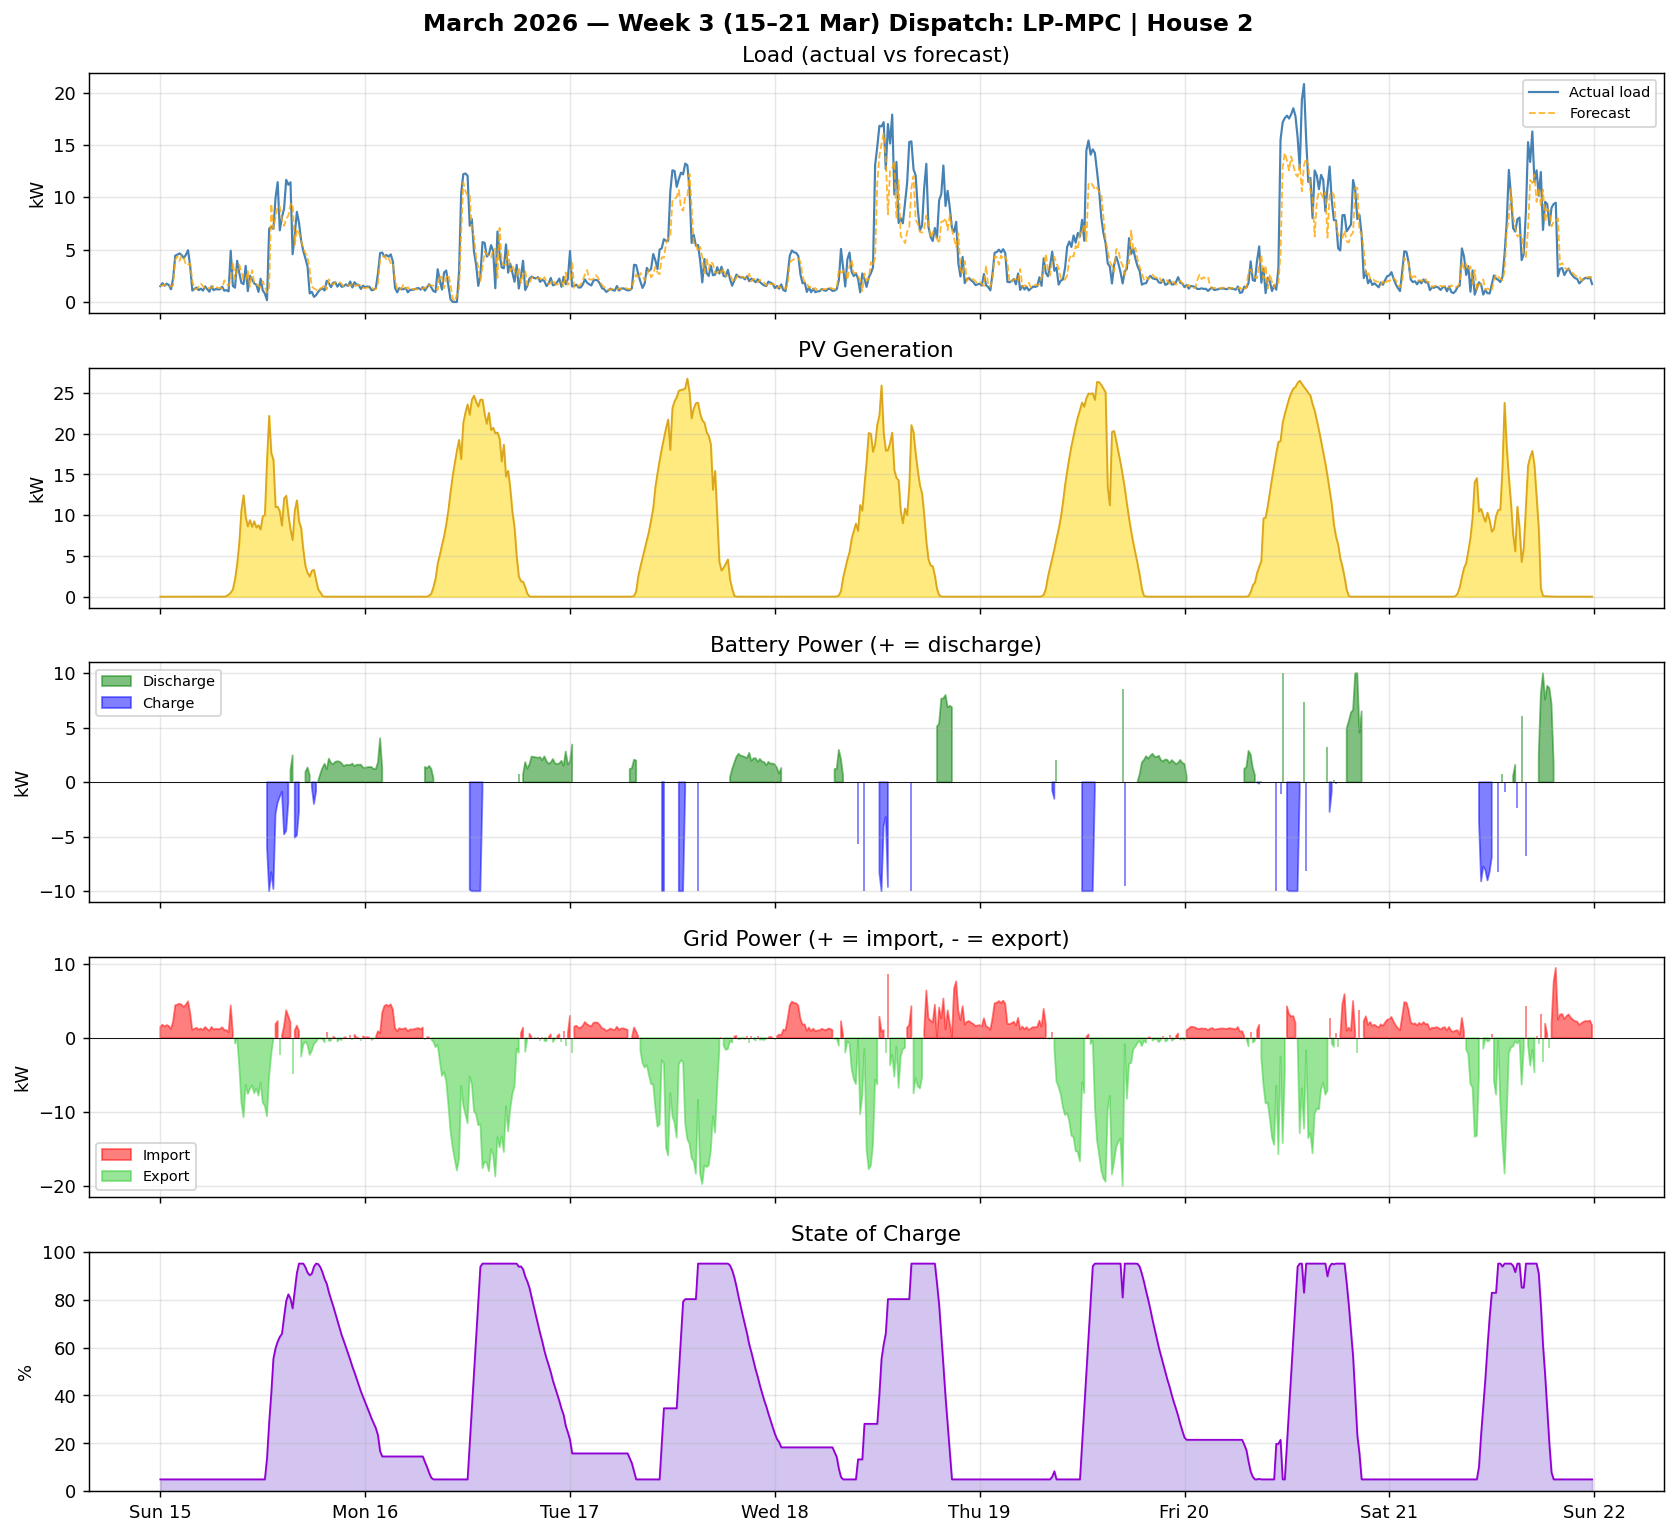
\includegraphics[width=0.92\textwidth, height=0.80\textheight,
                     keepaspectratio]{results/march_week3_house2_LP-MPC.png}
  \end{center}

  \vspace{-4pt}
  \begin{columns}[c]
    \begin{column}{0.32\textwidth}
      \centering\small
      \textcolor{energyblue}{\textbf{Panel 1--2:}} Load vs PV\\
      Spring surplus $\Rightarrow$ net export
    \end{column}
    \begin{column}{0.32\textwidth}
      \centering\small
      \textcolor{energyblue}{\textbf{Panel 3:}} Battery\\
      Charges at night (F3), discharges at peak (F1)
    \end{column}
    \begin{column}{0.32\textwidth}
      \centering\small
      \textcolor{energyblue}{\textbf{Panel 4--5:}} Grid \& SoC\\
      Correct sign convention verified
    \end{column}
  \end{columns}
\end{frame}

% ============================================================
%  SLIDE 4 — RESULTS TABLE
% ============================================================
\begin{frame}{Slide 4 \hfill \textcolor{gray}{\small$\approx$30 s}}
  \frametitle{Results: 2025 Annual Bill \& Savings}

  \begin{columns}[T]
    \begin{column}{0.52\textwidth}
      \begin{block}{Bill Comparison --- Full Year 2025}
        \renewcommand{\arraystretch}{1.3}
        \small
        \begin{tabular}{lcc}
          \toprule
          \textbf{Controller} & \textbf{Bill (\euro)} & \textbf{vs Baseline A} \\
          \midrule
          Baseline B (no battery) & 1\,598.28 & $+$31.1\,\% higher \\
          Baseline A (historical) & 1\,218.97 & reference \\
          \rowcolor{solaryellow!30}
          \textbf{LP-MPC (ours)}  & \textbf{1\,359.91} & $+$11.6\,\% higher \\
          \good{Oracle (perfect fcst)}   & \good{1\,212.56} & \good{$-$0.5\,\% better} \\
          \bottomrule
        \end{tabular}
      \end{block}

      \vspace{4pt}
      \begin{alertblock}{Key Gap Analysis}
        \small
        \begin{itemize}
          \item \good{Saves \euro238.37 (14.9\%) vs no-battery}
          \item Oracle $\Delta$ = \euro147.35 \textit{(cost of forecast error)}\\
                $\Rightarrow$ closing NRMSE gap would recover most savings
          \item Oracle \textbf{beats} Baseline A by \euro6.41\\
                $\Rightarrow$ LP formulation is near-optimal
        \end{itemize}
      \end{alertblock}
    \end{column}

    \begin{column}{0.44\textwidth}
      \begin{block}{Extension: Horizon Sensitivity (+5 pts)}
        \renewcommand{\arraystretch}{1.2}
        \small
        \begin{tabular}{cccr}
          \toprule
          $H$ & Time & Bill (\euro) & $\Delta$ vs $H$\,=\,4 \\
          \midrule
          4   & 1\,h   & 1\,601.37 & --- \\
          24  & 6\,h   & 1\,432.09 & $-$169 \\
          48  & 12\,h  & 1\,366.07 & $-$235 \\
          \rowcolor{solaryellow!30}
          \textbf{96} & \textbf{24\,h} & \textbf{1\,359.91} & $\mathbf{-241}$ \\
          \bottomrule
        \end{tabular}\\[4pt]
        \footnotesize
        Diminishing returns at $H$=96 (+\euro6 vs $H$=48)\\
        $\Rightarrow$ 24\,h is the recommended horizon
      \end{block}

      \vspace{4pt}
      \begin{exampleblock}{Billing Note}
        \small
        \textbf{Grid power uses actual load}, not forecast:\\
        $P_{\text{grid}} = L_{\text{true}} - P_{\text{PV}} - P_{\text{bat}}$\\
        Forecast error $\rightarrow$ bill impact, not data leak
      \end{exampleblock}
    \end{column}
  \end{columns}
\end{frame}

% ============================================================
%  SLIDE 5 — GENERALIZATION (DAY 2 SURPRISE DATASET)
% ============================================================
\begin{frame}{Slide 5 \hfill \textcolor{gray}{\small$\approx$30 s}}
  \frametitle{Generalization --- Day 2 Surprise Dataset}

  \begin{columns}[T]
    \begin{column}{0.48\textwidth}
      \begin{block}{NRMSE Comparison}
        \renewcommand{\arraystretch}{1.4}
        \begin{tabular}{lccc}
          \toprule
          \textbf{Dataset} & \textbf{RMSE} & \textbf{MAE} & \textbf{NRMSE} \\
          \midrule
          2025 test (House 1) & 0.68\,kW & 0.45\,kW &
            \textcolor{energyblue}{46.1\,\%} \\
          \rowcolor{solaryellow!30}
          \textbf{Day 2 (House 2)} & \textbf{1.30\,kW} & \textbf{0.79\,kW} &
            \good{\textbf{39.85\,\%}} \\
          \bottomrule
        \end{tabular}\\[4pt]
        \small\textit{Day 2 NRMSE \textbf{improves} by 6.3\,pp --- model
        generalises well to a new house.}
      \end{block}

      \vspace{6pt}
      \begin{block}{What Changed for Day 2}
        \small
        \begin{itemize}
          \item Different house: trained \textbf{only on 2nd dataset}\\
                (Nov 2024 -- Feb 2026, no cross-contamination)
          \item Same 43-feature pipeline; same hyperparameters
          \item Test period: \textbf{March 2026}
          \item More recent data (15 months) $\Rightarrow$ lower NRMSE
        \end{itemize}
      \end{block}
    \end{column}

    \begin{column}{0.48\textwidth}
      \begin{block}{Day 2 Controller Results --- March 2026}
        \renewcommand{\arraystretch}{1.3}
        \small
        \textit{Net exporter: bills shown as \textbf{net earnings} (\euro)}
        \begin{tabular}{lc}
          \toprule
          \textbf{Controller} & \textbf{Net Earning} \\
          \midrule
          Baseline A (historical) & \euro179.08 \\
          Baseline B (no battery) & \euro83.23 \\
          \rowcolor{solaryellow!30}
          \textbf{LP-MPC (ours)}  & \textbf{\euro138.21} \\
          Oracle (perfect fcst)   & \euro149.20 \\
          \midrule
          \good{Gain vs Baseline B} & \good{+\euro54.98 (+66\,\%)} \\
          Oracle gap              & \euro10.98 \\
          \bottomrule
        \end{tabular}
      \end{block}

      \vspace{4pt}
      \begin{exampleblock}{March 2026 Context}
        \small
        PV: \textbf{4\,039\,kWh} $\gg$ Load: \textbf{2\,423\,kWh}\\
        House earns from solar export all month\\
        LP-MPC shifts charge/discharge to maximise\\
        export revenue --- \textbf{+\euro54.98} vs no battery
      \end{exampleblock}
    \end{column}
  \end{columns}
\end{frame}

% ============================================================
%  SLIDE 6 — HARDEST PROBLEM & NEXT STEPS
% ============================================================
\begin{frame}{Slide 6 \hfill \textcolor{gray}{\small$\approx$30 s}}
  \frametitle{Hardest Problem \& What We Would Improve}

  \begin{columns}[T]
    \begin{column}{0.50\textwidth}
      \begin{alertblock}{[!] Hardest Bug: Energy Balance Sign Error}
        \small
        \textbf{The bug} --- LP constraint had wrong signs:
        \begin{align*}
          &\text{WRONG: } P_{\text{grid}}^+ - P_{\text{grid}}^-
            \;\bad{- P_d + P_c} = L - P_{\text{PV}} \\
          &\text{FIXED: } P_{\text{grid}}^+ - P_{\text{grid}}^-
            \;\good{+ P_d - P_c} = L - P_{\text{PV}}
        \end{align*}
        \textbf{Effect:} LP believed discharge \textit{increased} imports\\
        $\Rightarrow$ charged at peak, discharged at night\\
        $\Rightarrow$ \bad{Bill: \euro2\,096} (worse than both baselines!)

        \vspace{4pt}
        \textbf{Fix:} flip two coefficients in constraint matrix\\
        $\Rightarrow$ \good{Bill: \euro1\,360} --- correct dispatch immediately

        \vspace{4pt}
        \textbf{Lesson:} Validate controller direction first:\\
        \textit{does charging at night reduce the morning bill?}
      \end{alertblock}
    \end{column}

    \begin{column}{0.46\textwidth}
      \begin{block}{With One More Day\ldots}
        \small
        \renewcommand{\arraystretch}{1.15}
        \begin{tabular}{p{3.4cm}p{2.5cm}}
          \toprule
          \textbf{Improvement} & \textbf{Expected gain} \\
          \midrule
          Occupancy / smart-plug features & $-10$--$15$\,pp NRMSE \\
          Probabilistic MPC (scenario tree) & $-$\euro50--100 bill \\
          Day-ahead spot price forecast & market-dependent \\
          Horizon $H$=192 (48\,h) & small marginal \\
          Monthly model retraining & robustness \\
          \bottomrule
        \end{tabular}
      \end{block}

      \vspace{4pt}
      \begin{exampleblock}{Summary of Journey}
        \footnotesize
        \begin{tabular}{ll}
          NRMSE start (long lags only): & \bad{67.6\,\%} \\
          + short lags (\texttt{lag\_1..lag\_16}): & 48.6\,\% \\
          + momentum + expanded features: & \good{46.1\,\%} \\[3pt]
          Bill before sign fix: & \bad{\euro2\,096} \\
          Bill after sign fix: & \good{\euro1\,360} \\
          Oracle (best possible): & \good{\euro1\,213} \\
        \end{tabular}
      \end{exampleblock}
    \end{column}
  \end{columns}
\end{frame}

% ─────────────────────────────────────────────────────────────
\end{document}
